\section{La technique}

\subsection{Outils}
\begin{frame}
  \frametitle{\color{white} Outils de développement}
  \begin{block}{Langage}
    \begin{itemize}
      \item C++ 11.
      \hfill
      
\includegraphics[scale=.07]{cpp-logo.png}
      \item Qt 5.
      \hfill
      
\includegraphics[scale=.008]{Qt-logo.png}
    \end{itemize}
  \end{block}
  \begin{block}{Pourquoi le C++ 11 ?}
    \begin{itemize}
      \item Rapidité d'exécution.
      \item Communication simplifiée avec GPG.
      \item Langage natif de Qt.
    \end{itemize}
  \end{block}
  \begin{block}{Pourquoi Qt 5 ?}
    \begin{itemize}
      \item Cadriciel multiplate-forme.
      \item KDE est basé sur ce cadriciel.
    \end{itemize}
  \end{block}
\end{frame}

\subsection{Maquette}
\begin{frame}
  \frametitle{\color{white} Maquette}
  \begin{block}{Livrables}
    \begin{itemize}
      \item Livrable 1 : Gestion des clefs, vue des commandes.
      \item Livrable 2 : Éditeur/opérations cryptographiques.
      \item Livrable 3 : Toile de confiance.
    \end{itemize}
  \end{block}
  \begin{center}
    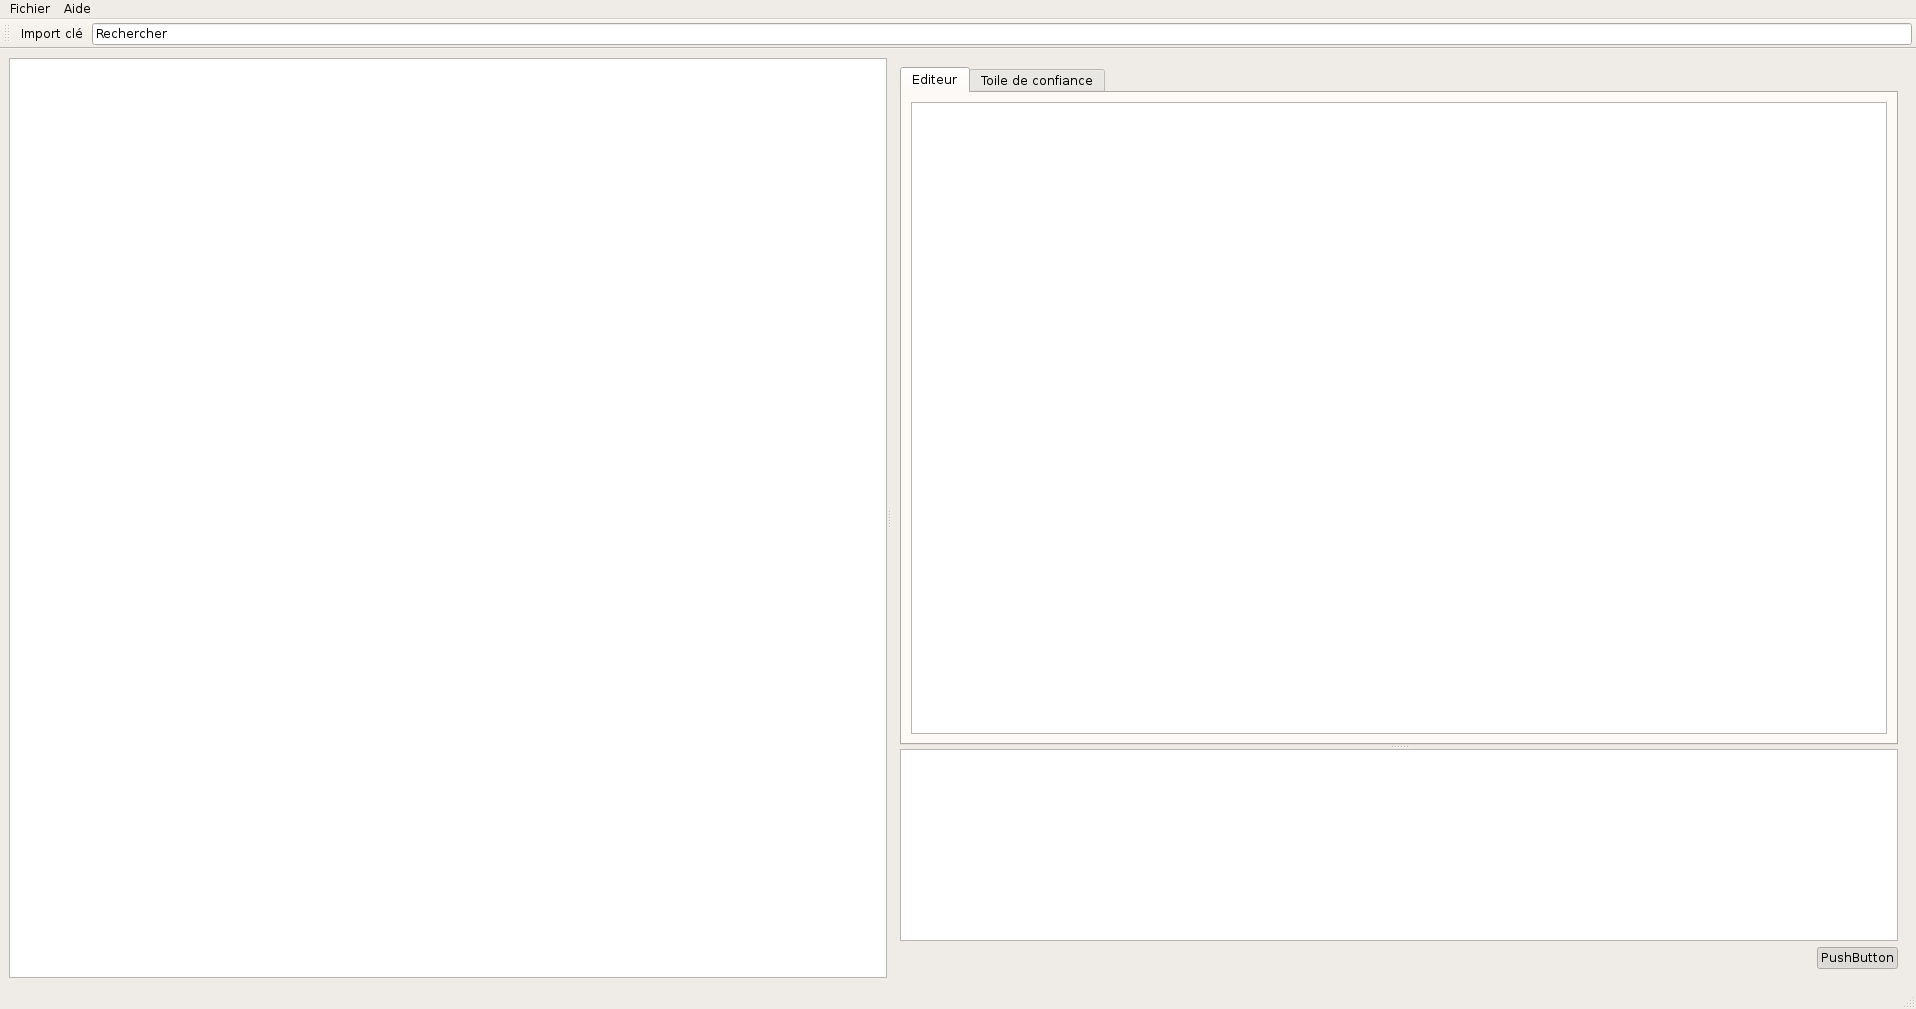
\includegraphics[scale=.14]{maquette.png}
  \end{center}
\end{frame}

\subsection{Procédés de gestion}
\begin{frame}
  \frametitle{\color{white} Procédés de gestion}
  \hfill
  
\includegraphics[scale=.05]{git-logo.png}
  \begin{center}
    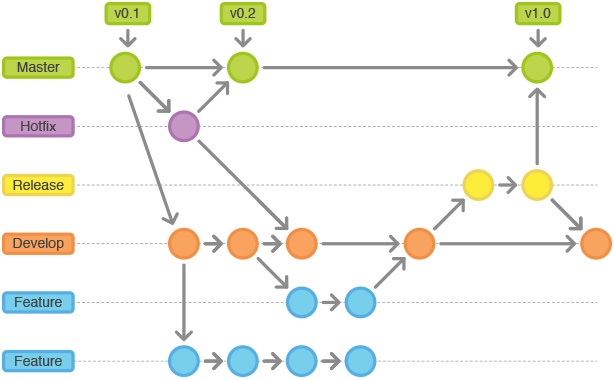
\includegraphics[scale=.45]{git_workflow}
  \end{center}
\end{frame}

\subsection{Risque}
\begin{frame}
  \frametitle{\color{white} Maîtrise des outils}
  \begin{block}{Prévention}
    \begin{itemize}
      \item Réalisation de séances de programmation C++/Qt.
      \item Réalisation de séances de découverte d'OpenPGP avec GnuPG.
    \end{itemize}
  \end{block}
  \begin{block}{Actions}
    \begin{itemize}
      \item Séances d'approfondissement des outils en continu.
      \item Ré-attribution des rôles en fonction des difficultés rencontrées.
    \end{itemize}
  \end{block}
\end{frame}

